We propose here a likely schedule for the project, shown in 2 GANTT charts. The chart are divided in a temporal basis to enhance readability. The first chart includes the Requirements Analysis and Design phases, whereas the second one includes the Development and Deployment phases. The total schedule duration is almost 7 months, that is very near the project effort estimation from the previous chapter. 
\bigbreak
The colors in the chart have the following meaning: 
\begin{itemize}
\item \textbf{GREEN: } Macro-phase duration
\item \textbf{BLUE: } Meeting with PowerEni
\item \textbf{ORANGE: } Single task
\item \textbf{GRAY: } System is online
\end{itemize}

\begin{figure}
  \centering
  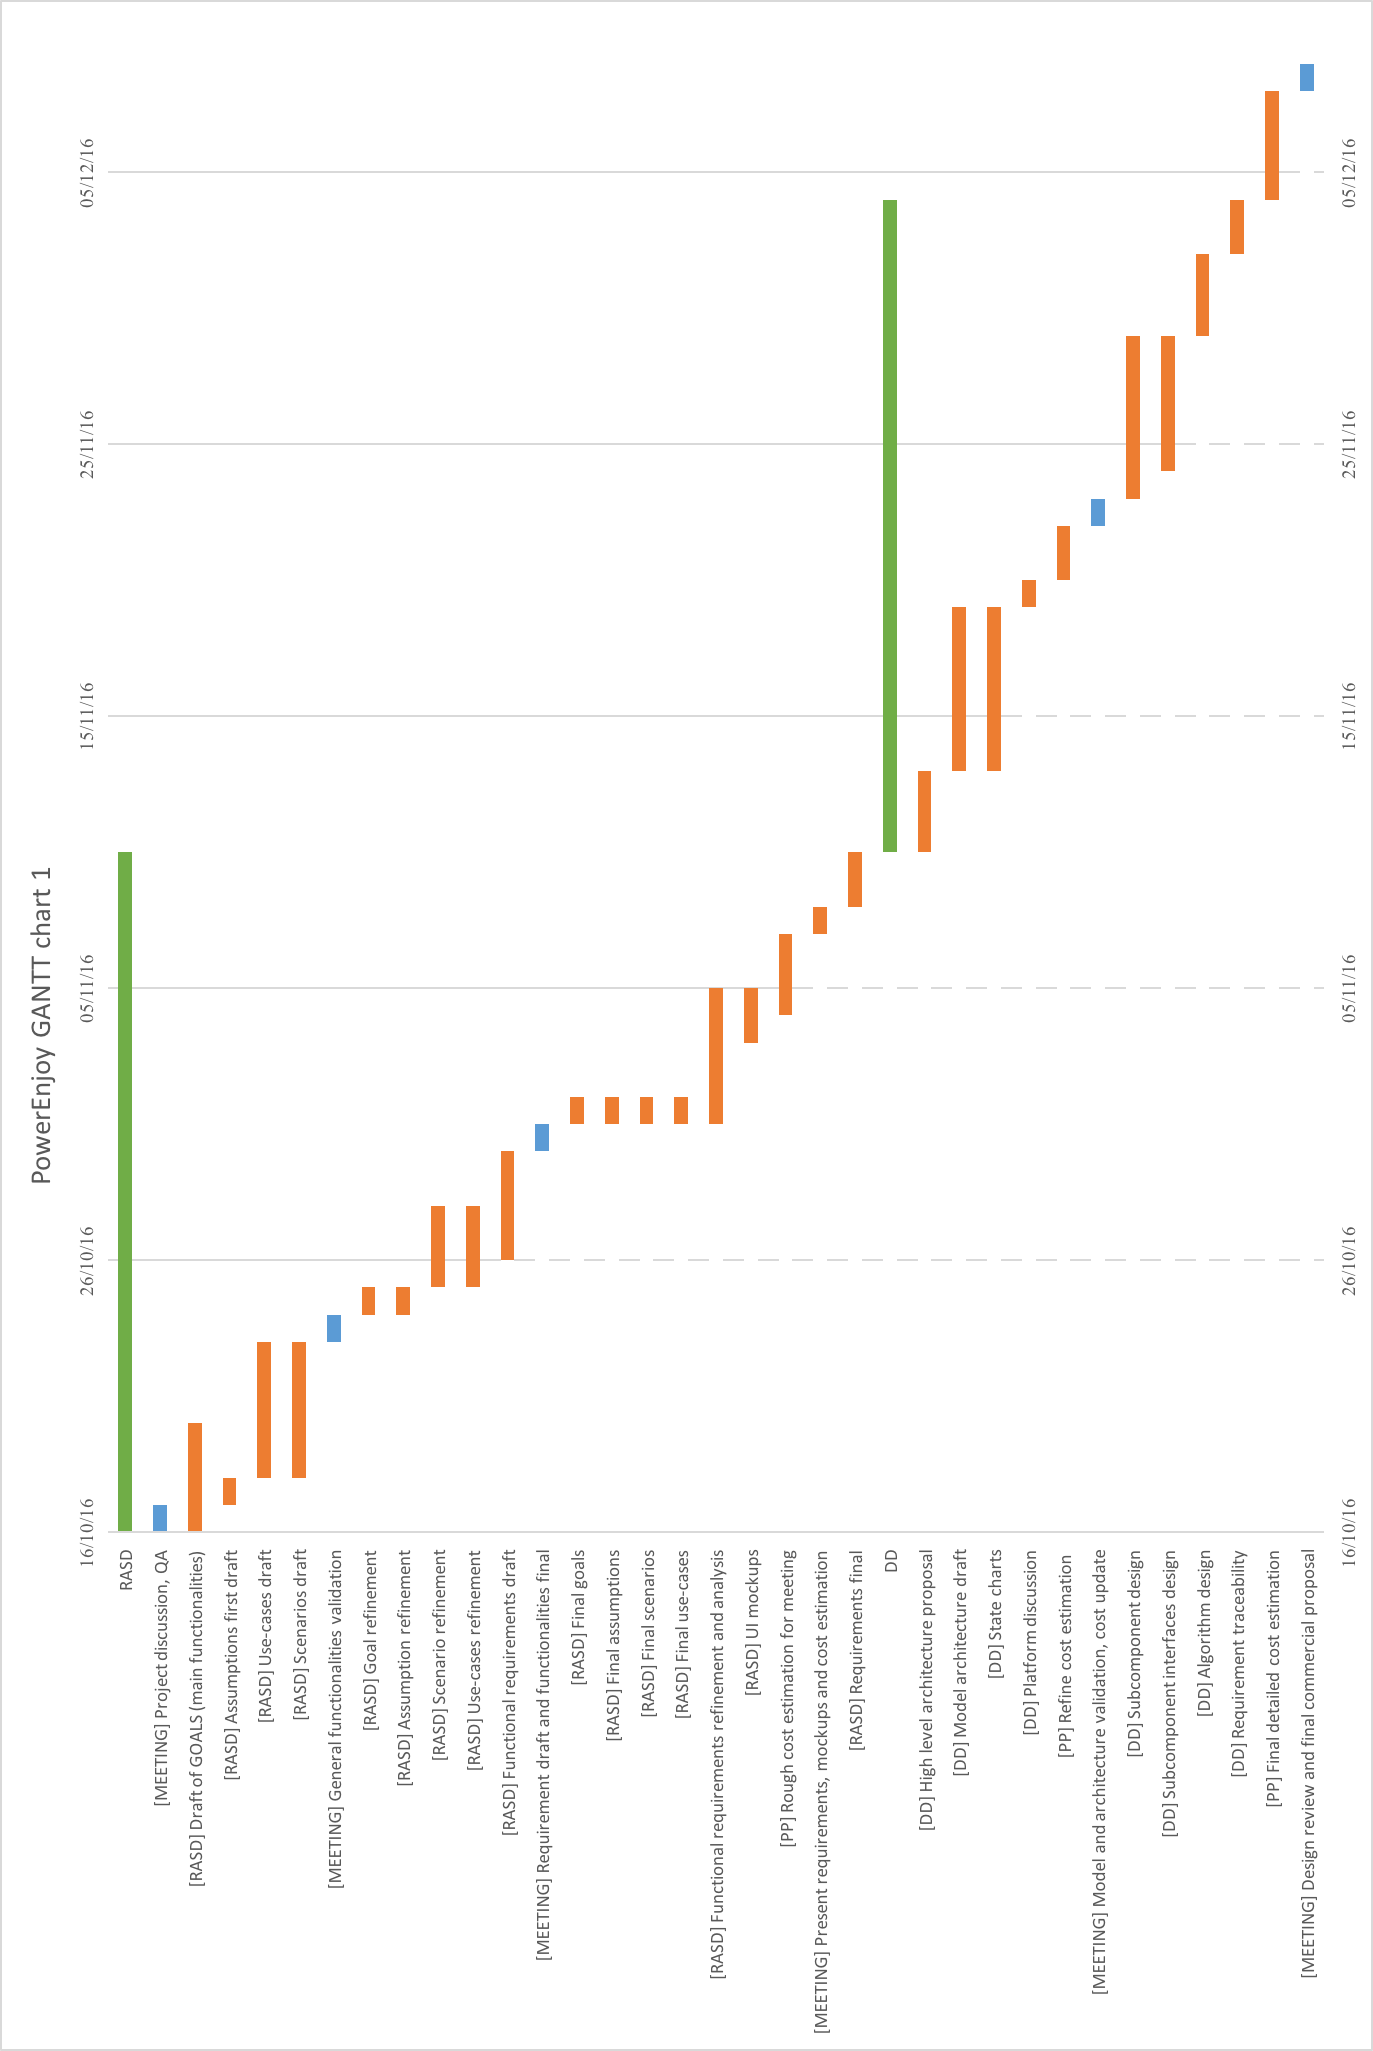
\includegraphics[width=1.0\textwidth]{gantt1}
  \caption{GANTT chart of first period from 16/10/2016 to 09/12/2016.}
\end{figure}

\begin{figure}
  \centering
  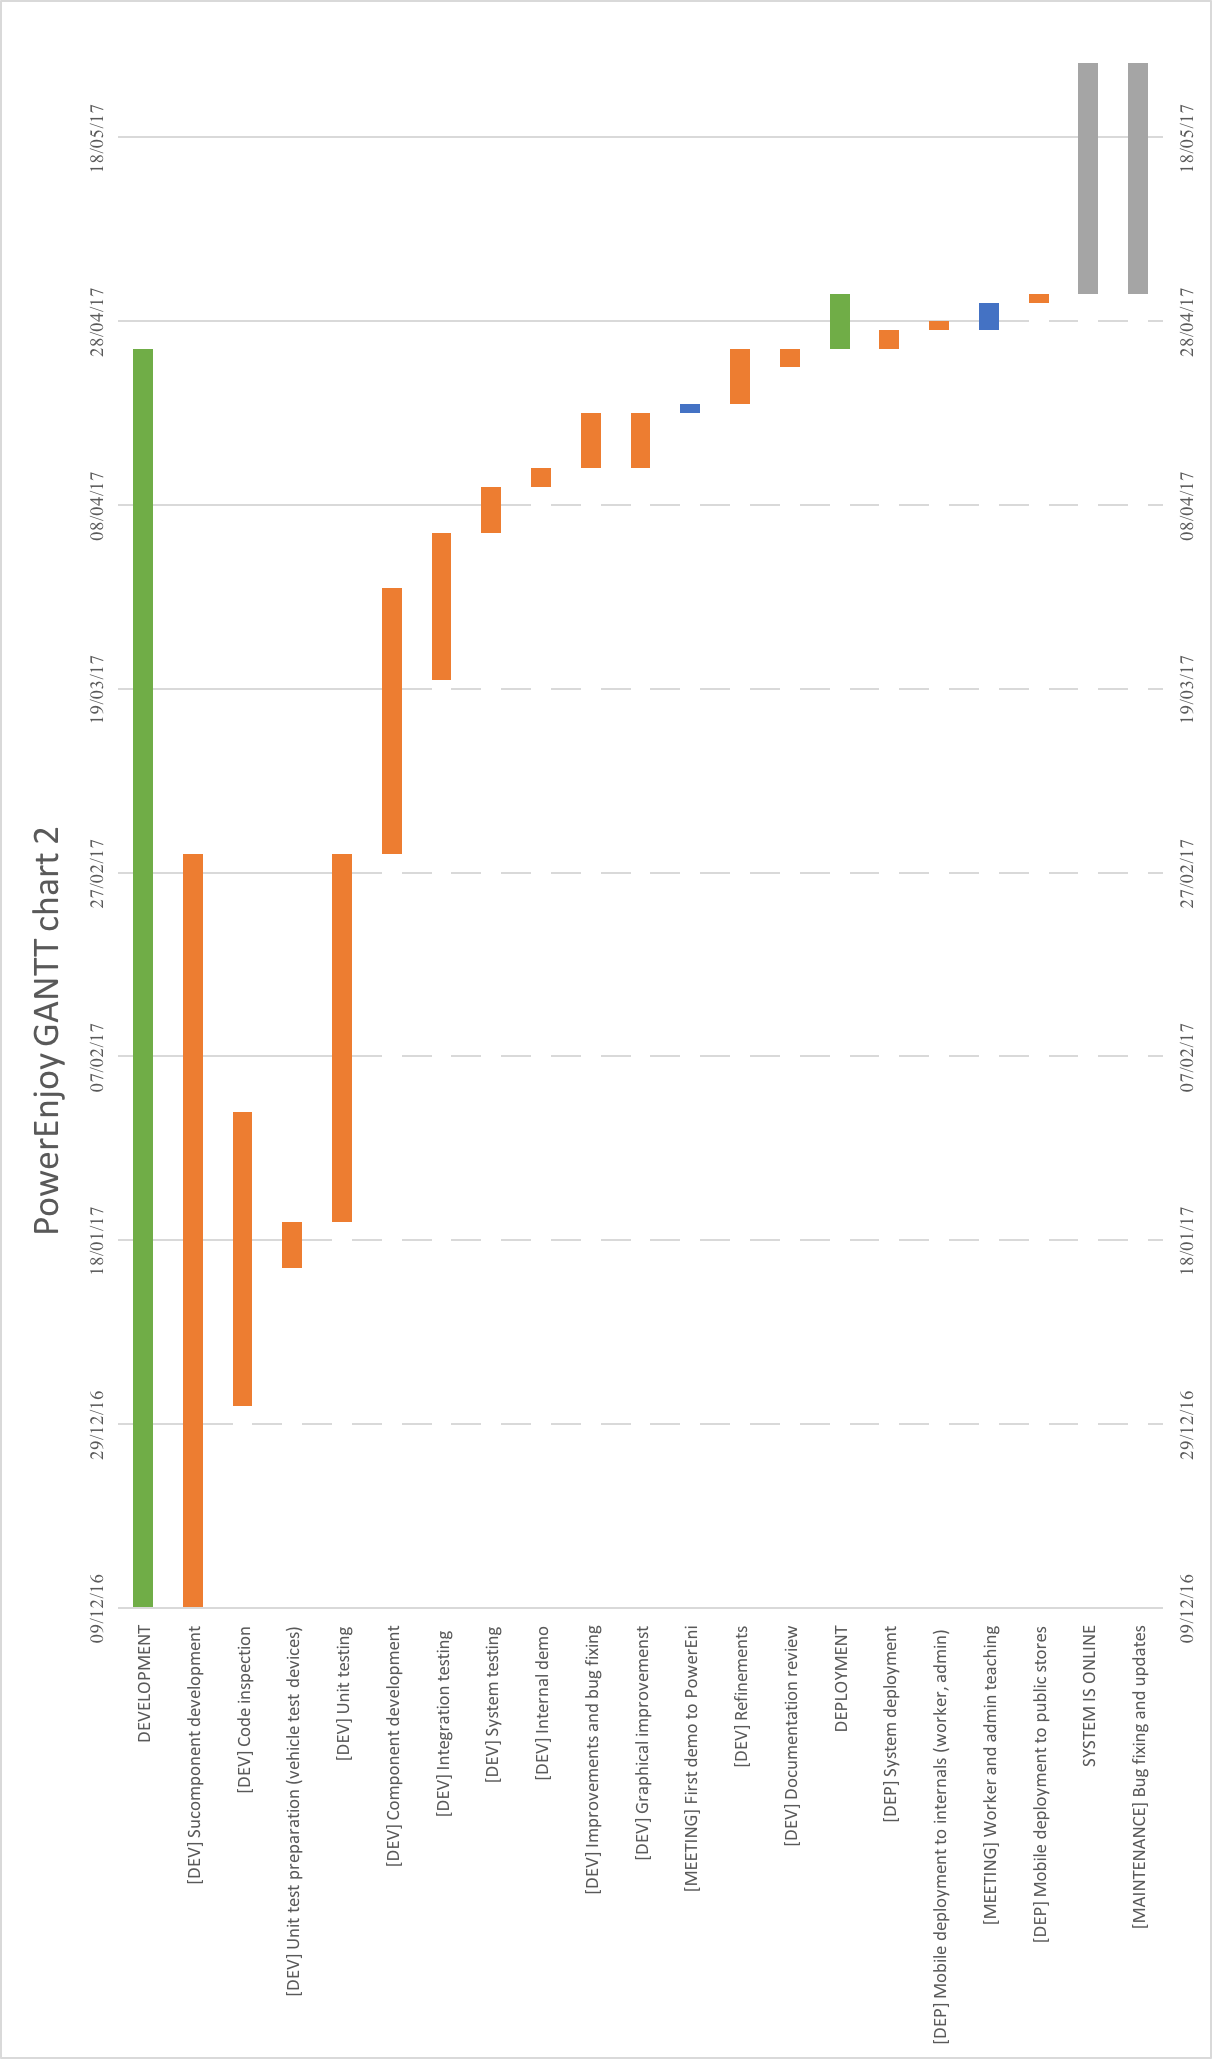
\includegraphics[width=1.0\textwidth]{gantt2}
  \caption{GANTT chart of second period from 09/12/2016 to 01/05/2017.}
\end{figure}